
\section{Introduction}\label{sec:1}
\hspace{0.5cm}
Un nouveau cadre pour les calculs neutroniques de base développé à EDF R\&D, dans
le département de SINETICS (SImulation NEutronique, Technologie de l'Information,
Calcul Scientifique) est basé sur la résolution de l'équation de Boltzmann
(ou une approximation) pour les neutrons.\\
Cette équation nécessite en entrée des sections efficaces qui modélisent les
interactions entre les neutrons induits par la fission et les noyaux provenant
soit du combustible soit du modérateur. \\

Ces sections efficaces (au nombre de plusieurs milliers) dépendent
de $d$ paramètres locaux (dits paramètres de rétroaction), tels que la densité de l'eau,
la concentration en bore, la température du carburant, le brûlage du combustible, etc.
Elles sont stockées dans des «bibliothèque nucléaire» et doivent être consultées
régulièrement tout au long de la simulation quand les paramètres de rétroaction évoluent. \\

Dans le cadre d’une thèse CIFRE \cite{These} qui vient d’être soutenue au
Laboratoire J.-L. Lions, une nouvelle méthode \cite{Luu} basée sur l’utilisation
de bases tensorielles a été développé. Ces méthodes utilisent des fonctions directionnelles
adaptées aux fonctions qu’on veut représenter et qui permet de diminuer le stockage, le coût
des calculs pour reconstruire les sections efficaces avec une très grande précision. \\

L'objectif du stage est de comparer cette étude avec une approche alternative (méthodes parcimonieuses)
proposée récemment au Laboratoire J.-L. Lions par Albert Cohen \cite{Albert}.
Le stage porte sur la mise en œuvre de ces méthodes parcimonieuses pour le cas particulier de l'approximation
des sections efficaces. Il s'agit pour certaines d'entre elles de méthodes non-intrusives (donc basées sur
des évaluations obtenues par un code qui peut être vu comme une boite noire,
ce qui est bien adapté à la situation). Elles font appel à des techniques de représentations parcimonieuses
dans le but de tirer parti des anisotropies potentielles dans la fonction qu'on veut capturer
(certaines variables pouvant en particulier être plus sensibles que d'autres) et des propriétés
de régularité en fonction des différentes variables.

\paragraph{Mots clés:} Sections efficaces, méthodes parcimonieuses, interpolation multivariée ...

%-------------------------------------------------------------------------------------------------------------%
\newpage
\section{Présentation de la structure d’accueil}\label{sec:2}
\hspace{0.5cm}
Le laboratoire, créé en 1969, porte le nom de son fondateur Jacques-Louis Lions.
Il s’agit maintenant d’une unité de recherche conjointe à l’Université Pierre et Marie Curie,
à l’université Paris Diderot et au Centre National de la Recherche Scientifique. \\

Le Laboratoire Jacques-Louis Lions constitue le plus grand laboratoire de France et l’un
des principaux au monde pour la formation et la recherche en mathématiques appliquées. \\

Il accueille l’activité de deux masters deuxième année ce qui représente une centaine d’étudiants.
Ses axes de recherche recouvrent l’analyse, la modélisation et le calcul scientifique haute
performance de phénomènes représentés par des équations aux dérivées partielles.
Fort d’environ 100 enseignants-chercheurs, chercheurs, ingénieurs, personnels administratifs
permanents ou émérites, et d’autant de doctorants ou post-doctorants, le LJLL collabore avec
le monde économique et avec d’autres domaines scientifiques à travers un large spectre
d’applications: dynamique des fluides; physique, mécanique et chimie théoriques; contrôle,
optimisation et finance; médecine et biologie; traitement du signal et des données.
\begin{center}
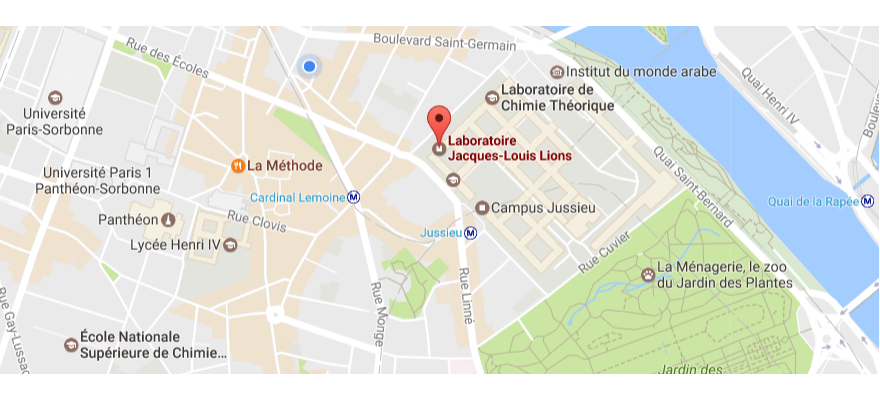
\includegraphics[height=8cm,width=0.9\linewidth]{images/Localisation.png}
\captionof{figure}{Localisation de la structure d'accueil}
\end{center}

%-------------------------------------------------------------------------------------------------------------%
\newpage
